\documentclass[12pt]{article}
\usepackage{fancyhdr}
\usepackage[letterpaper, margin=1in]{geometry}
%\usepackage{indentfirst}
\usepackage{graphicx}
\usepackage{amsmath}
\usepackage{amssymb}
\usepackage{siunitx}
\sisetup{detect-weight=true, detect-family=true} % makes siunitx follow font formatting like bold, italic, etc.
\usepackage{cancel}
\usepackage{isotope}
\usepackage{listings}
\usepackage[dvipsnames,table]{xcolor}
\usepackage{xspace}
\usepackage{booktabs} % makes tables pretty
\usepackage{longtable} % for long tables
\usepackage{multirow} % makes tables pretty
\usepackage{multicol} % makes tables pretty
\usepackage{setspace}
\usepackage{subcaption}
\usepackage{hyperref}
\usepackage{cleveref}
\newcommand{\creflastconjunction}{, and\nobreakspace} % adds oxford comma to cleveref
\usepackage[utf8]{inputenc}
\usepackage{textcomp}
\usepackage{titlesec}
\usepackage{svg}
\usepackage{pdflscape} % makes pages landscape
\usepackage{mathtools}
\usepackage{enumitem}
\usepackage[T1]{fontenc}




% si units stuff
\DeclareSIUnit\year{yr}
\DeclareSIUnit\hour{hr}
\DeclareSIUnit\mole{mol}

% fancy header stuff
\usepackage{fancyhdr}
\pagestyle{fancy}

\setlength{\headheight}{28pt}
\lhead{NSE 565 \\ Winter 2022}
\chead{Homework 1\\}
\rhead{Austin Warren\\Due February 11, 2022}

% bib if needed
\bibliographystyle{ieeetr}

\begin{document}

%%%%%%%%%%%%%%%%%%%%%%%%%%%%%%%%%%
\section{Methods}

\begin{equation}
    \int\limits_S \rho \overline{u} \phi \cdot \overline{n} dS = \int\limits_S \Gamma \frac{\partial \phi}{\partial x} \cdot \overline{n} dS + \int\limits_V q_{\phi} dV
    \label{eq:transport}
\end{equation}

We can approximate the two surface integrals as follows:
\begin{equation*}
    \int\limits_S \rho \overline{u} \phi \cdot \overline{n} dS = \left( \rho\underline(u) S\phi \right)_{i+1} - \left( \rho\underline(u) S\phi \right)_{i-1}\:,
\end{equation*}
and
\begin{equation*}
    \int\limits_S \Gamma \frac{\partial \phi}{\partial x} \cdot \overline{n} dS = \left( \Gamma S \frac{\partial \phi}{\partial x} \right)_{i+1} - \left( \Gamma S \frac{\partial \phi}{\partial x} \right)_{i-1}\:.
\end{equation*}
We can approximate the volume integral as follows:
\begin{equation*}
    \int\limits_V q_{\phi} dV = \overline{q} V\:.
\end{equation*}
If we assume $S$ is constant our transport equation becomes:
\begin{equation*}
    \left( \rho \overline(u) \phi \right)_{i+1} - \left( \rho \overline(u) \phi \right)_{i-1} = \left( \Gamma \frac{\partial \phi}{\partial x} \right)_{i+1} - \left( \Gamma \frac{\partial \phi}{\partial x} \right)_{i-1} + \overline{q} V\:.
\end{equation*}
We can apply the Central Differencing Scheme approximations:
\begin{align*}
    \phi_{i+1} &= \frac{\phi_{I+1} + \phi_{I}}{2} & \phi_{i-1} &= \frac{\phi_{I-1} + \phi_{I}}{2} \\
    \left(\frac{\partial \phi}{\partial x}\right)_{i+1} &= \frac{\phi_{I+1} - \phi_{I}}{\delta x} & \left(\frac{\partial \phi}{\partial x}\right)_{i-1} &= \frac{\phi_{I} - \phi_{I-1}}{\delta x}
\end{align*}
The transport equation now looks like:
\begin{equation*}
    \left(\frac{\rho \overline{u}}{2}\right)_{i+1} \left( \phi_{I+1} + \phi_{I} \right) - \left(\frac{\rho \overline{u}}{2}\right)_{i-1} \left( \phi_{I-1} + \phi_{I} \right) = \frac{\Gamma}{\Delta x} \left( \phi_{I+1} - \phi_{I} \right) - \frac{\Gamma}{\Delta x} \left( \phi_{I} - \phi_{I-1} \right) + \overline{q}_{I}\: \Delta x\:.
\end{equation*}
For this problem, the density and velocity are constant throughout the geometry. We can group terms and get the transport equation in a useful form to sovle.
\begin{equation}
    \left[ -\frac{\rho \overline{u}}{2} - \frac{\Gamma}{\Delta x} \right] \phi_{I-1} + \left[ \frac{2\Gamma}{\Delta x} \right] \phi_{I} + \left[ \frac{\rho \overline{u}}{2} - \frac{\Gamma}{\Delta x} \right] \phi_{I+1} = \overline{q}_{I}\: \Delta x
    \label{eq:grouped}
\end{equation}
We can rewrite this equation as:
\begin{equation}
    a_{I}\phi_{I-1} + b_{I}\phi_{I} + c_{I}\phi_{I+1} = Q_{I}\:.
    \label{eq:coef}
\end{equation}
This equation works for middle nodes, but the edge nodes do not have enough neighbor nodes. The first node does not have another node to the left of it ($I-1$), so we have to only use the value at the left edge, which is $\phi_{L}$. This gives us:
\begin{equation}
    \left[ \left( \frac{\rho \overline{u}}{2} \right)_{i+1} + \frac{3 \Gamma}{\Delta x} \right]\phi_{I} + \left[ \left( \frac{\rho \overline{u}}{2} \right)_{i+1} - \frac{\Gamma}{\Delta x} \right]\phi_{I+1} = \overline{q}_{I}\: \Delta x + \left( \rho \overline{u} \phi \right)_{L} + \frac{2\Gamma}{\Delta x}\phi_L\:,
    \label{eq:node 1 grouped}
\end{equation}
which gives us an equation of the form:
\begin{equation}
    b_1 \phi_1 + c_1 \phi_2 = Q_1\:.
    \label{eq:node 1 coef}
\end{equation}
If we do the same on the right side we get:

\begin{equation}
    \left[ -\left( \frac{\rho \overline{u}}{2} \right)_{i-1} + \frac{3 \Gamma}{\Delta x} \right]\phi_{I-1} + \left[ -\left( \frac{\rho \overline{u}}{2} \right)_{i-1} - \frac{\Gamma}{\Delta x} \right]\phi_{I} = \overline{q}_{I}\: \Delta x - \left( \rho \overline{u} \phi \right)_{R} + \frac{2\Gamma}{\Delta x}\phi_R\:,
    \label{eq:node N grouped}
\end{equation}
and:
\begin{equation}
    a_N \phi_{N-1} + b_{N} \phi_N = Q_N\:.
    \label{eq:node N coef}
\end{equation}


%%%%%%%%%%%%%%%%%%%%%%%%%%%%%%%%%%
\section{Results}
    % plots
    \Cref{fig:case1} shows the two solutions for Case 1: 5 control volumes and $\overline{u}=\SI{0.1}{\meter\per\second}$.
    \Cref{fig:case2} shows the two solutions for Case 2: 5 control volumes and $\overline{u}=\SI{2.5}{\meter\per\second}$.
    \Cref{fig:case3} shows the two solutions for Case 3: 20 control volumes and $\overline{u}=\SI{2.5}{\meter\per\second}$.
    \begin{figure}[htbp]
        \centering
        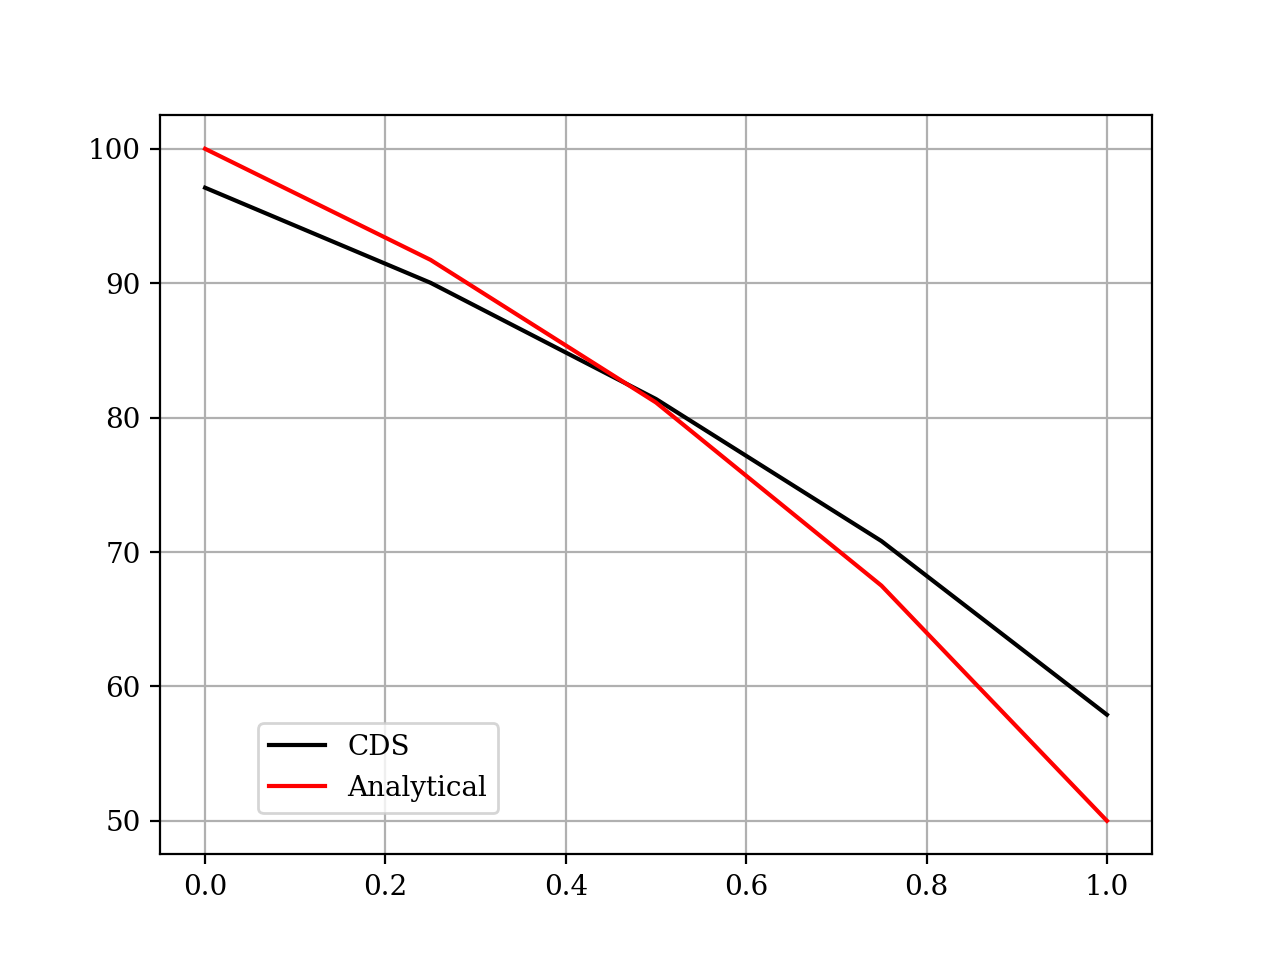
\includegraphics[width=\textwidth]{plots/graph_case1.png}
        \caption{Central Difference Scheme and Analytical Solutions for Case 1.}
        \label{fig:case1}
    \end{figure}

    
    \begin{figure}[htbp]
        \centering
        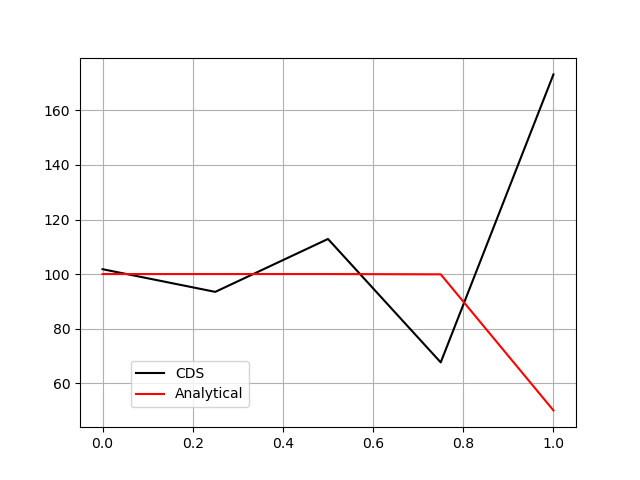
\includegraphics[width=\textwidth]{plots/graph_case2.png}
        \caption{Central Difference Scheme and Analytical Solutions for Case 2.}
        \label{fig:case2}
    \end{figure}

    
    \begin{figure}[htbp]
        \centering
        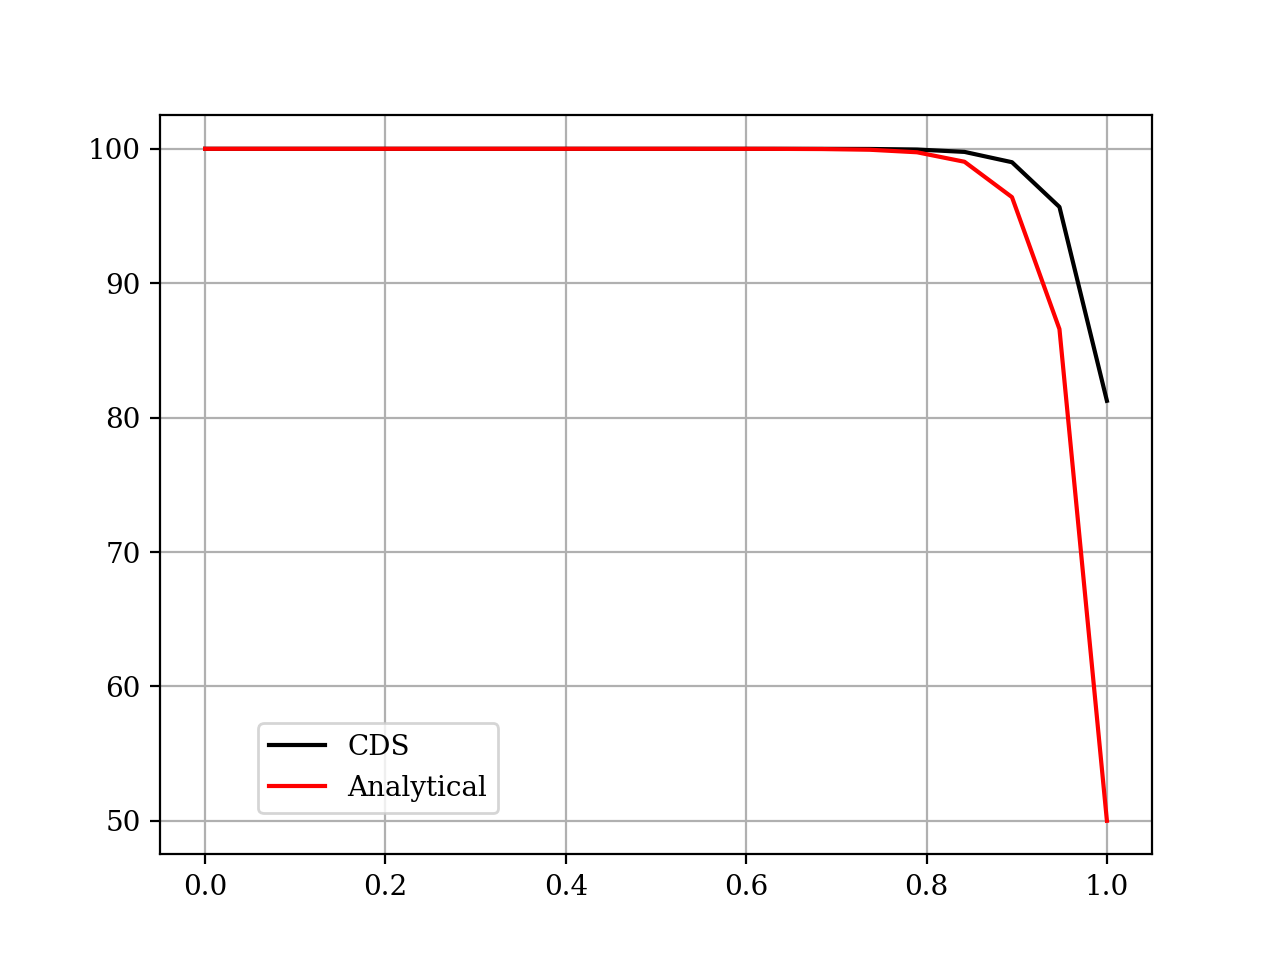
\includegraphics[width=\textwidth]{plots/graph_case3.png}
        \caption{Central Difference Scheme and Analytical Solutions for Case 3.}
        \label{fig:case3}
    \end{figure}

    \clearpage
    % table
    \Cref{tab:error} lists the error values calculated for each case.
    \begin{table}[htbp]
	 \centering
	 \caption{Error values for each case.}
	 \begin{tabublar}{cc}
		 \toprule
		 Case & Error \\ 
		 \midrule 
		 1 & 3.213926974817029 \\ 
		 2 & 35.33997019002361 \\ 
		 3 & 2.1977755170786173 \\ 
		 \bottomrule 
	 \end{tabular} 
	 \label{tab:error} 
\end{table}

    

%%%%%%%%%%%%%%%%%%%%%%%%%%%%%%%%%%
\section{Discussion}
We can use the Peclet number to see how stable each solution should be to determine if the solutions perform how we expect them to.
\begin{equation}
    Pe = \frac{\rho \overline{u}}{\Gamma / \Delta x}
\end{equation}
For this problem, we want $Pe<2$. \Cref{tab:Pe} shows the Peclet numbers for each case. As we can see, the second case does not meet the criteria for stability, so we expect the numerical solution to be unstable. The other two solutions are expected to be stable and they are. Also, the solutions go from a value of 100 on the left towards a value of 50 on the right, which we would expect from the boundary conditions.
\begin{table}[htbp]
	 \centering
	 \caption{Peclet number for each case.}
	 \begin{tabular}{cc}
		 \toprule
		 Case & $Pe$ \\ 
		 \midrule 
		 1 & 0.20000000000000004 \\ 
		 2 & 5.0 \\ 
		 3 & 1.25 \\ 
		 \bottomrule 
	 \end{tabular} 
	 \label{tab:Pe} 
\end{table}


\end{document}